\documentclass{article}
\usepackage{graphicx}
\usepackage{subcaption}
\usepackage[margin=1.0in]{geometry}
\setlength\parindent{0pt}
\usepackage[titletoc]{appendix}


\begin{document}

\title{Visualising Live Code Study Report}
\author{Arrian Purcell}

\maketitle

\begin{figure}
\centering
\begin{subfigure}{.5\textwidth}
    \centering
    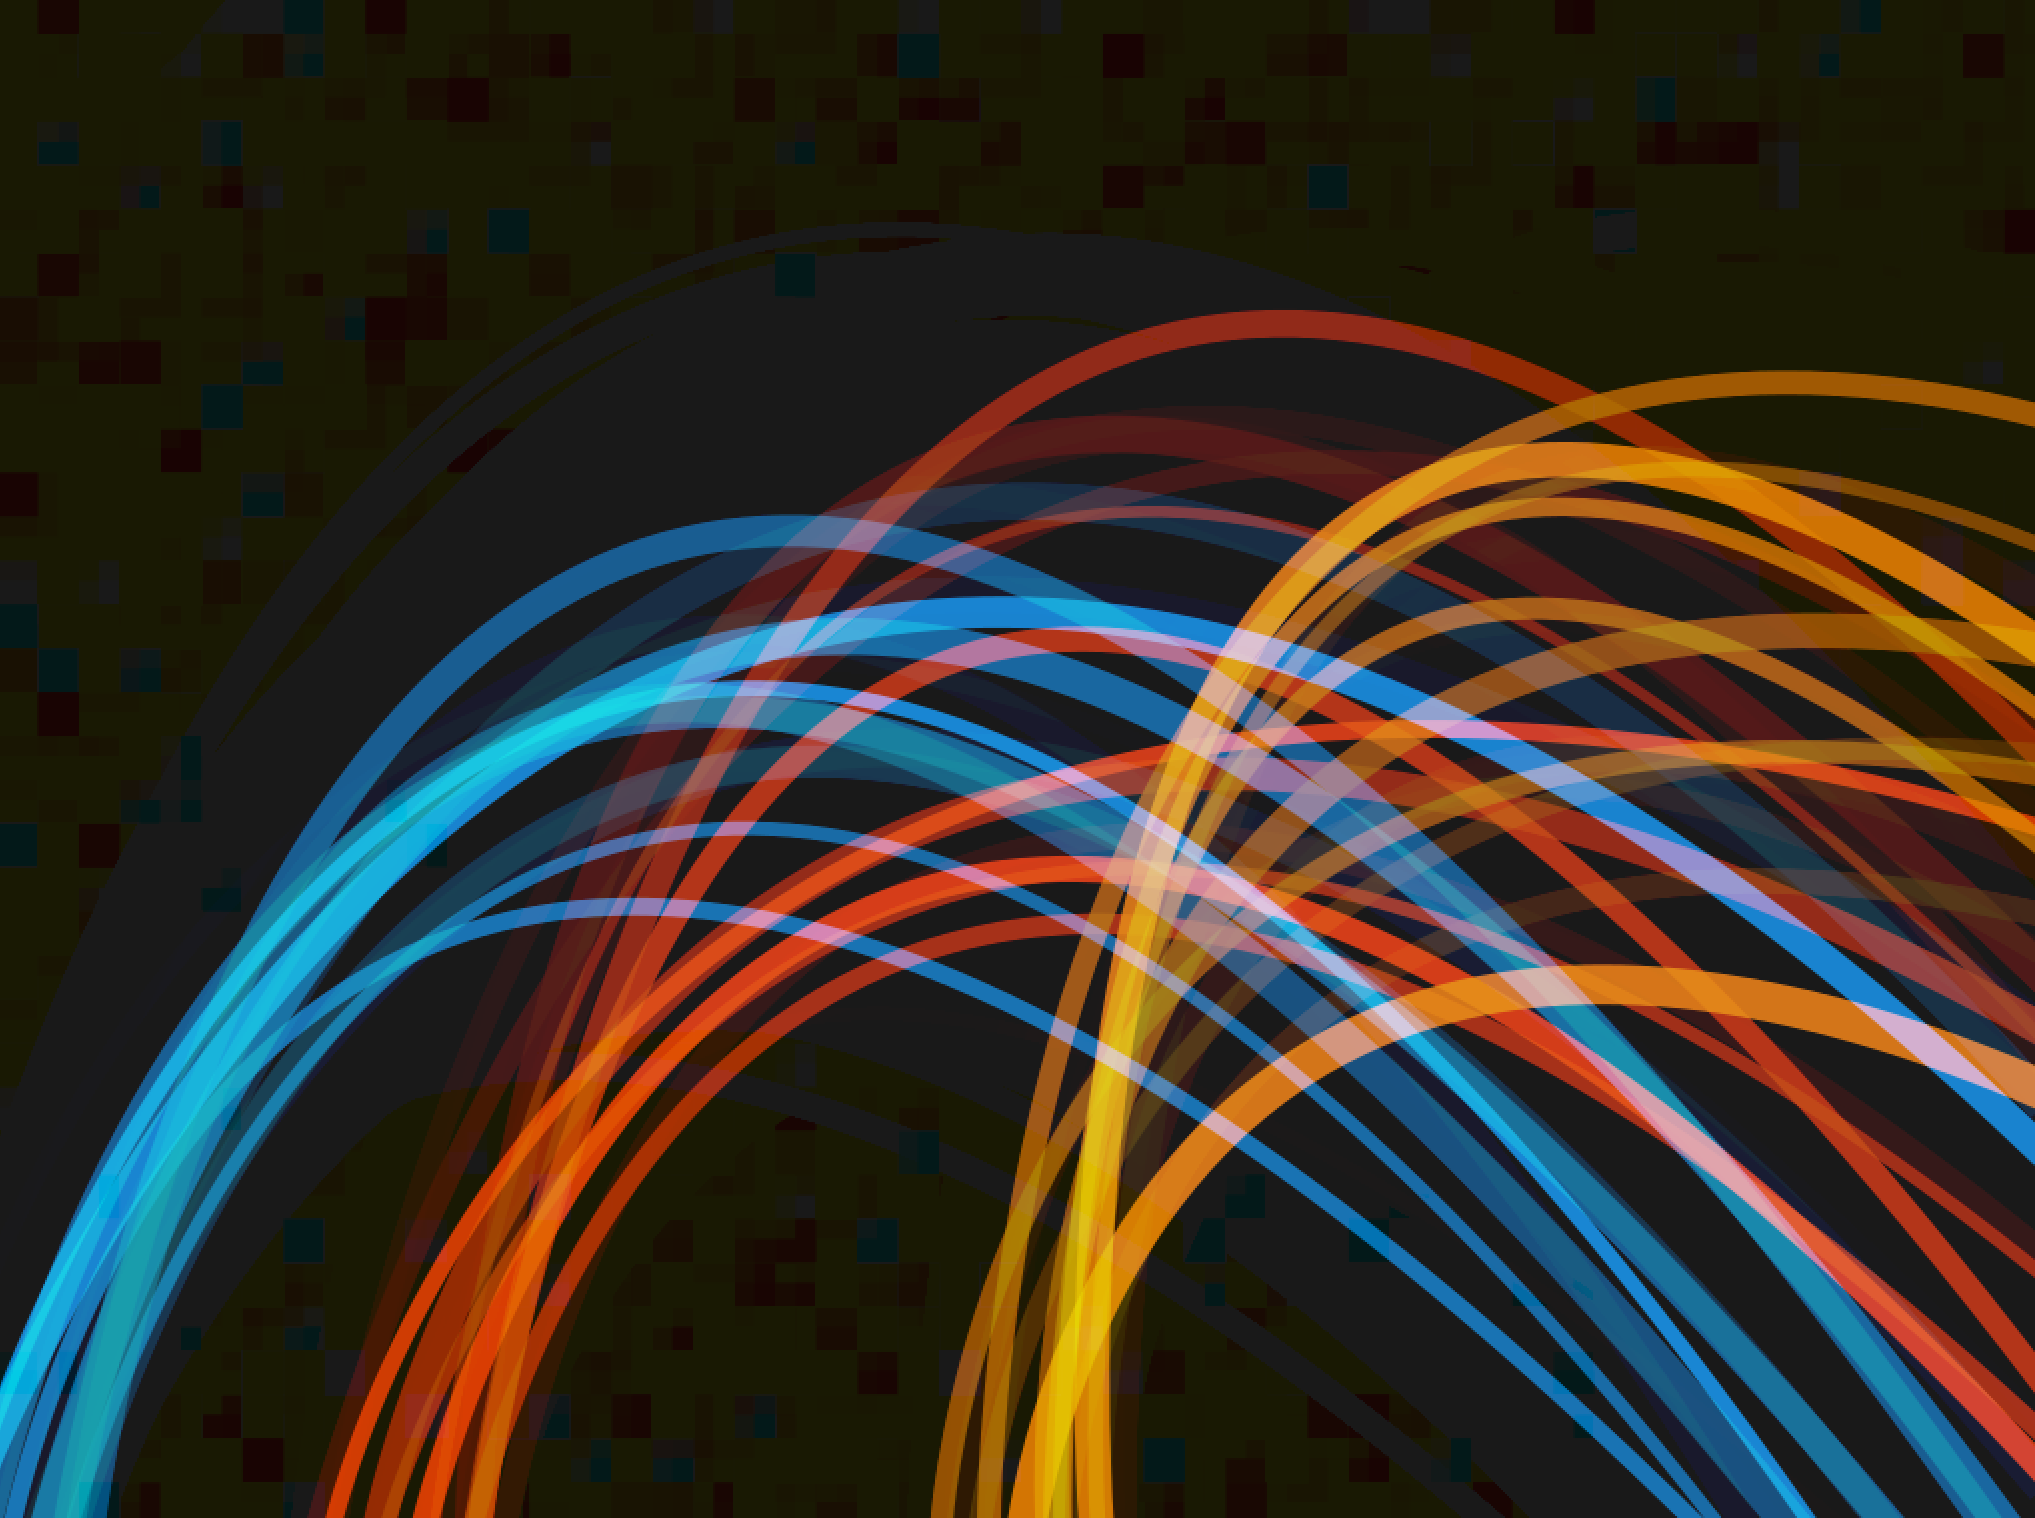
\includegraphics[width=0.9\linewidth]{aesthetic-vis.png}
    \caption{Aesthetic Visualisation}
    \label{avis}
\end{subfigure}%
\begin{subfigure}{.5\textwidth}
    \centering
    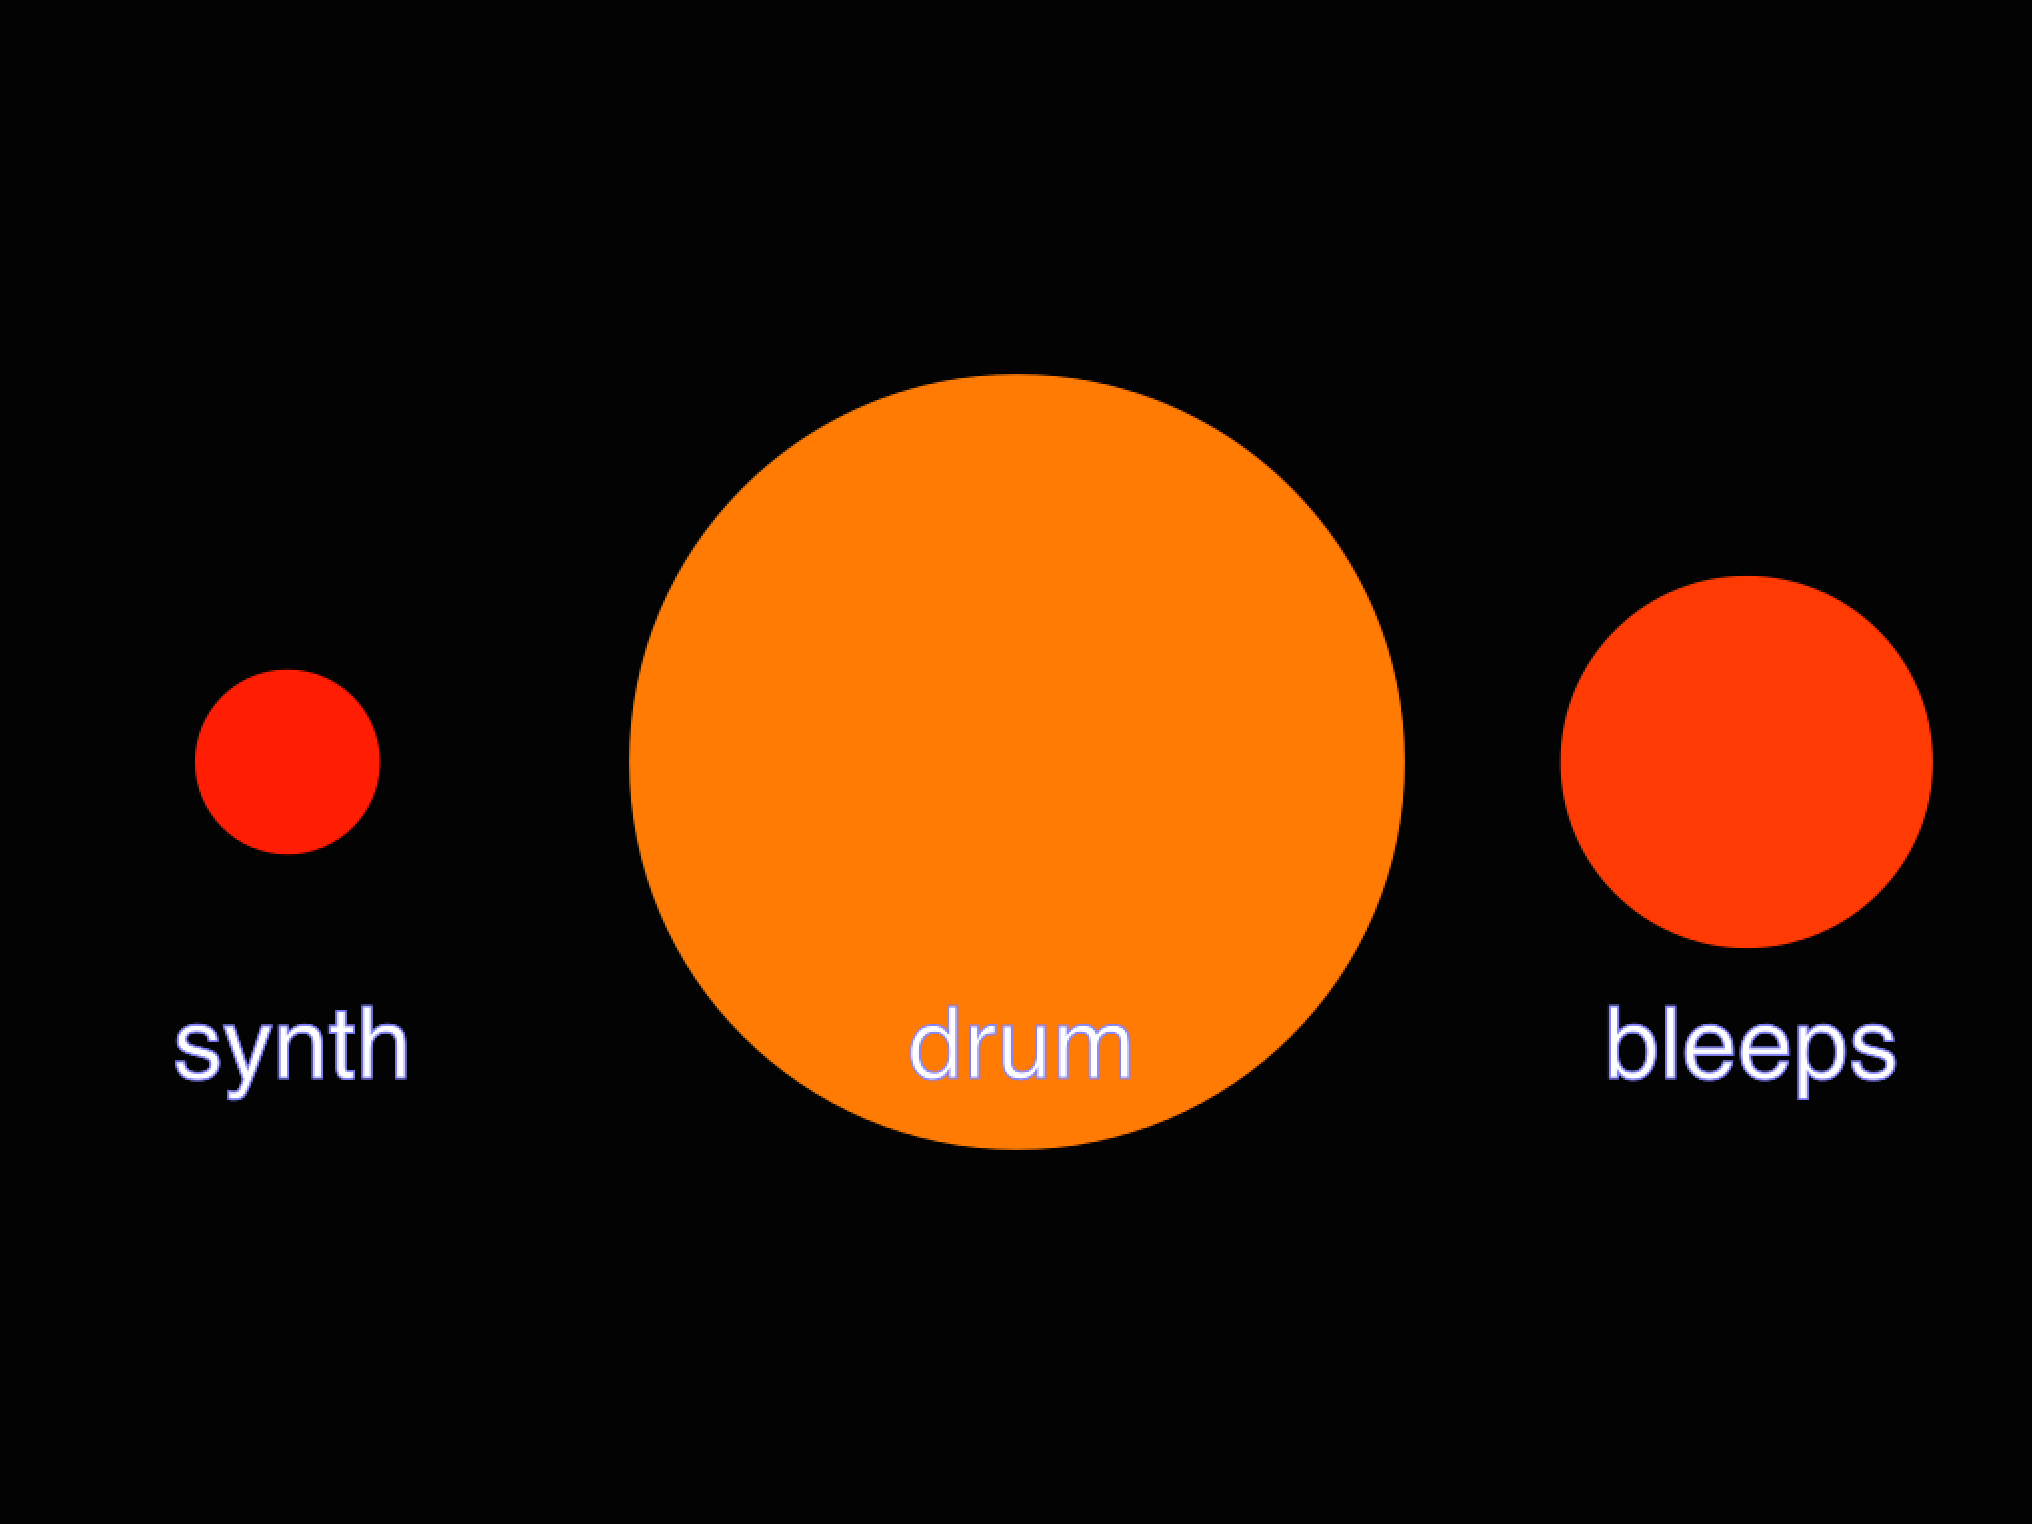
\includegraphics[width=0.9\linewidth]{didactic-vis.png}
    \caption{Didactic Visualisation}
    \label{dvis}
\end{subfigure}
\caption{Visualisation Examples}
\end{figure}

For most of its history programming code has been displayed as simple text due to the expressiveness of this format and despite its inefficiencies. It is only recently, due to ever increasing programming language complexity and increasing computational power, that code annotations and syntax highlighting have become more commonplace. Nevertheless, these visual enhancements rarely provide information beyond the basic grammar of the language they are intended to augment. The limitations of this approach are becoming ever more apparent as programming languages and interactive programming environments move towards the need for real-time comprehension.\\

[talk about interactive programming environments and real-time comprehension]\\

The human brain is highly proficient in pattern recognition (Ware, 2013) and there is evidence to suggest that visualisations can take advantage of this proficiency to enhance understanding (Najjar, 1998). From this, one could potentially conclude that visualisations could be further applied to aid in the process of real-time code comprehension within the space of interactive programming environments [citation needed].\\

[how can the problem be approached?]\\

To this end, two code visualisations have been analysed in a live coding context to determine effective presentational and educational features. The two visualisations evaluated included a visualisation targeting aesthetic appeal and a visualisation with a more didactic approach. The goal was to determine differences and desirable aspects of the two visualisation approaches in order to inform future live coding visualisations.\\

The set of didactic visualisations predominantly focussed on the relationship between the live coding active processes and their behaviour. The visualisations prominently displaying the names of the active functions with visual indication of the number of functions running and their callback time. Bright colours and solid shapes were used to ensure constant visibility and communicate the intention of the underlying code. An example of this approach can be seen in Figure \ref{dvis}. Overall, four visualisations were presented with each introduced depending on the number of active functions.\\

The set of aesthetic visualisations focussed less on the programmatic aspects of the live coding performance, rather intending to provide additional visual interest to the projected code. To this end, more variety was used in visual structure and colour. An example of this approach can be seen in Figure \ref{avis}. Again, four visualisations were presented, varying which visualisation was displayed depending on the number of active functions.\\

[literature supporting the visualisations presented]\\

visual variables...\\

hierarchy of graphical elements...\\

visualisation analysis model...\\

[summary]\\

[link to study method]\\

\section{Method}
Two sets of visualisations were presented to an audience during a live coding performance and surveys were distributed. The performance was run as two ten minute improvised songs with each song demonstrating one of the two experimental visualisation conditions, either the didactic condition or the aesthetic condition. The experiment was run twice, with two separate participant groups, swapping the order in which the two sets of visualisations were presented to the audience.\\

The audience members completed a survey consisting of four sections over the course of the performance. These sections included a demographic information section, opinion of the first visualisation, opinion of the second visualisation and a section investigating the audience's overall opinion of the performance. The sections regarding the visualisations predominantly focussed on the enjoyment and understanding related to the visualisation while the final section focussed on eliciting potential improvements.

After explaining to the participants the structure of the experiment and allowing the participants to complete the initial demographic section of a survey, the live coder began the first performance utilising one of the two visualisations. Following this first set, the second section of the survey was conducted. A second set was then played using the alternative visualisation. Following this second set, the same survey questions were administered again, again asking the participants specifics about their enjoyment and understanding related to the specific visualisation demonstrated. A final survey question was then asked relating to their opinion regarding the whole performance and suggested improvements.

\section{Participants}

A total of 41 participants took part in the study. Over the two performances, 19 participants observed the first performance and 22 participants observed the second performance. The demographic makeup between the two performances was very similar.\\

$66\%$ of the participants stated that they were male (see Figure \ref{genderdistribution}) and most participants were aged between 18 and 32 ($76\%$, see Figure \ref{agedistribution}). As the study was conducted within the Computer Science Department, a large proportion of the participants were experienced with programming with $90\%$ having current or previous experience with it. Nevertheless, only $15\%$ of participants had previous experience with any of the Lisp style of languages.\\

Of the participants, $68\%$ stated that they listened to a large amount of music (see Figure \ref{musicdistribution}) though only about $15\%$ of participants stated that they played and instrument or sung regularly (see Figure \ref{instrumentdistribution}). Only $22\%$ of participants had seen a live coding performance before.\\

\begin{figure}[t]
\centering
\begin{subfigure}{.5\textwidth}
    \centering
    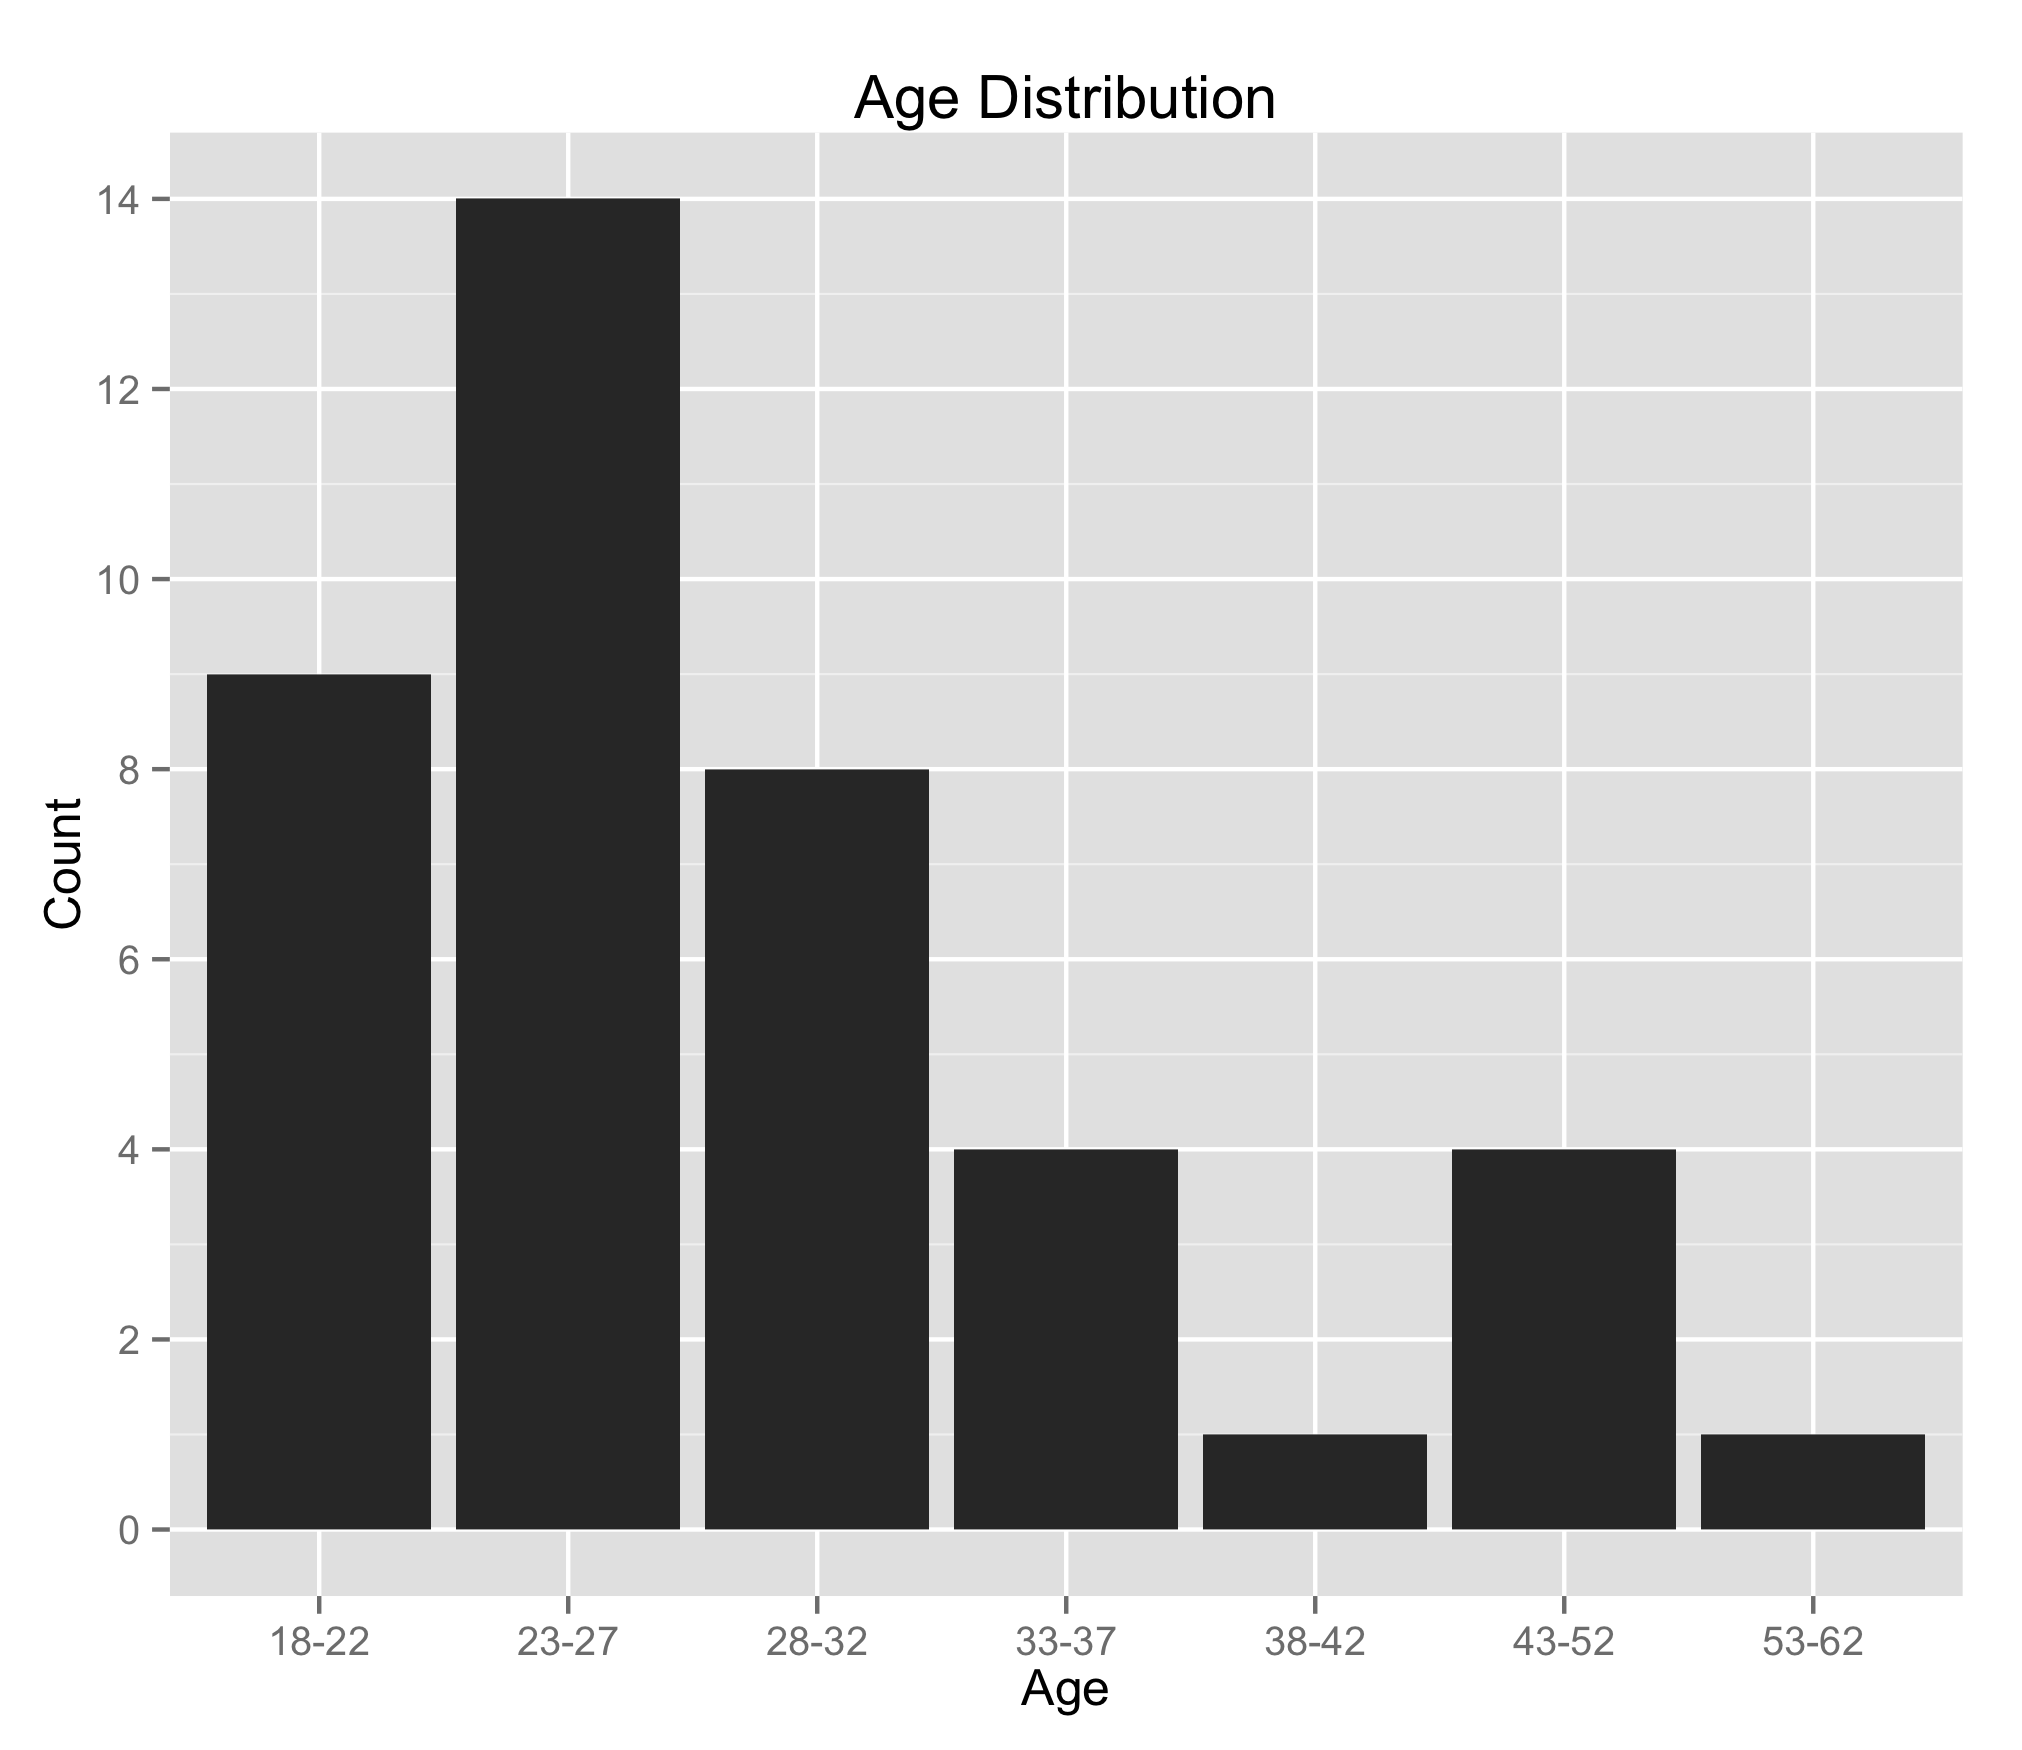
\includegraphics[width=1.0\linewidth]{graphs/age.png}
    \caption{Age Distribution}
    \label{agedistribution}
\end{subfigure}%
\begin{subfigure}{.5\textwidth}
    \centering
    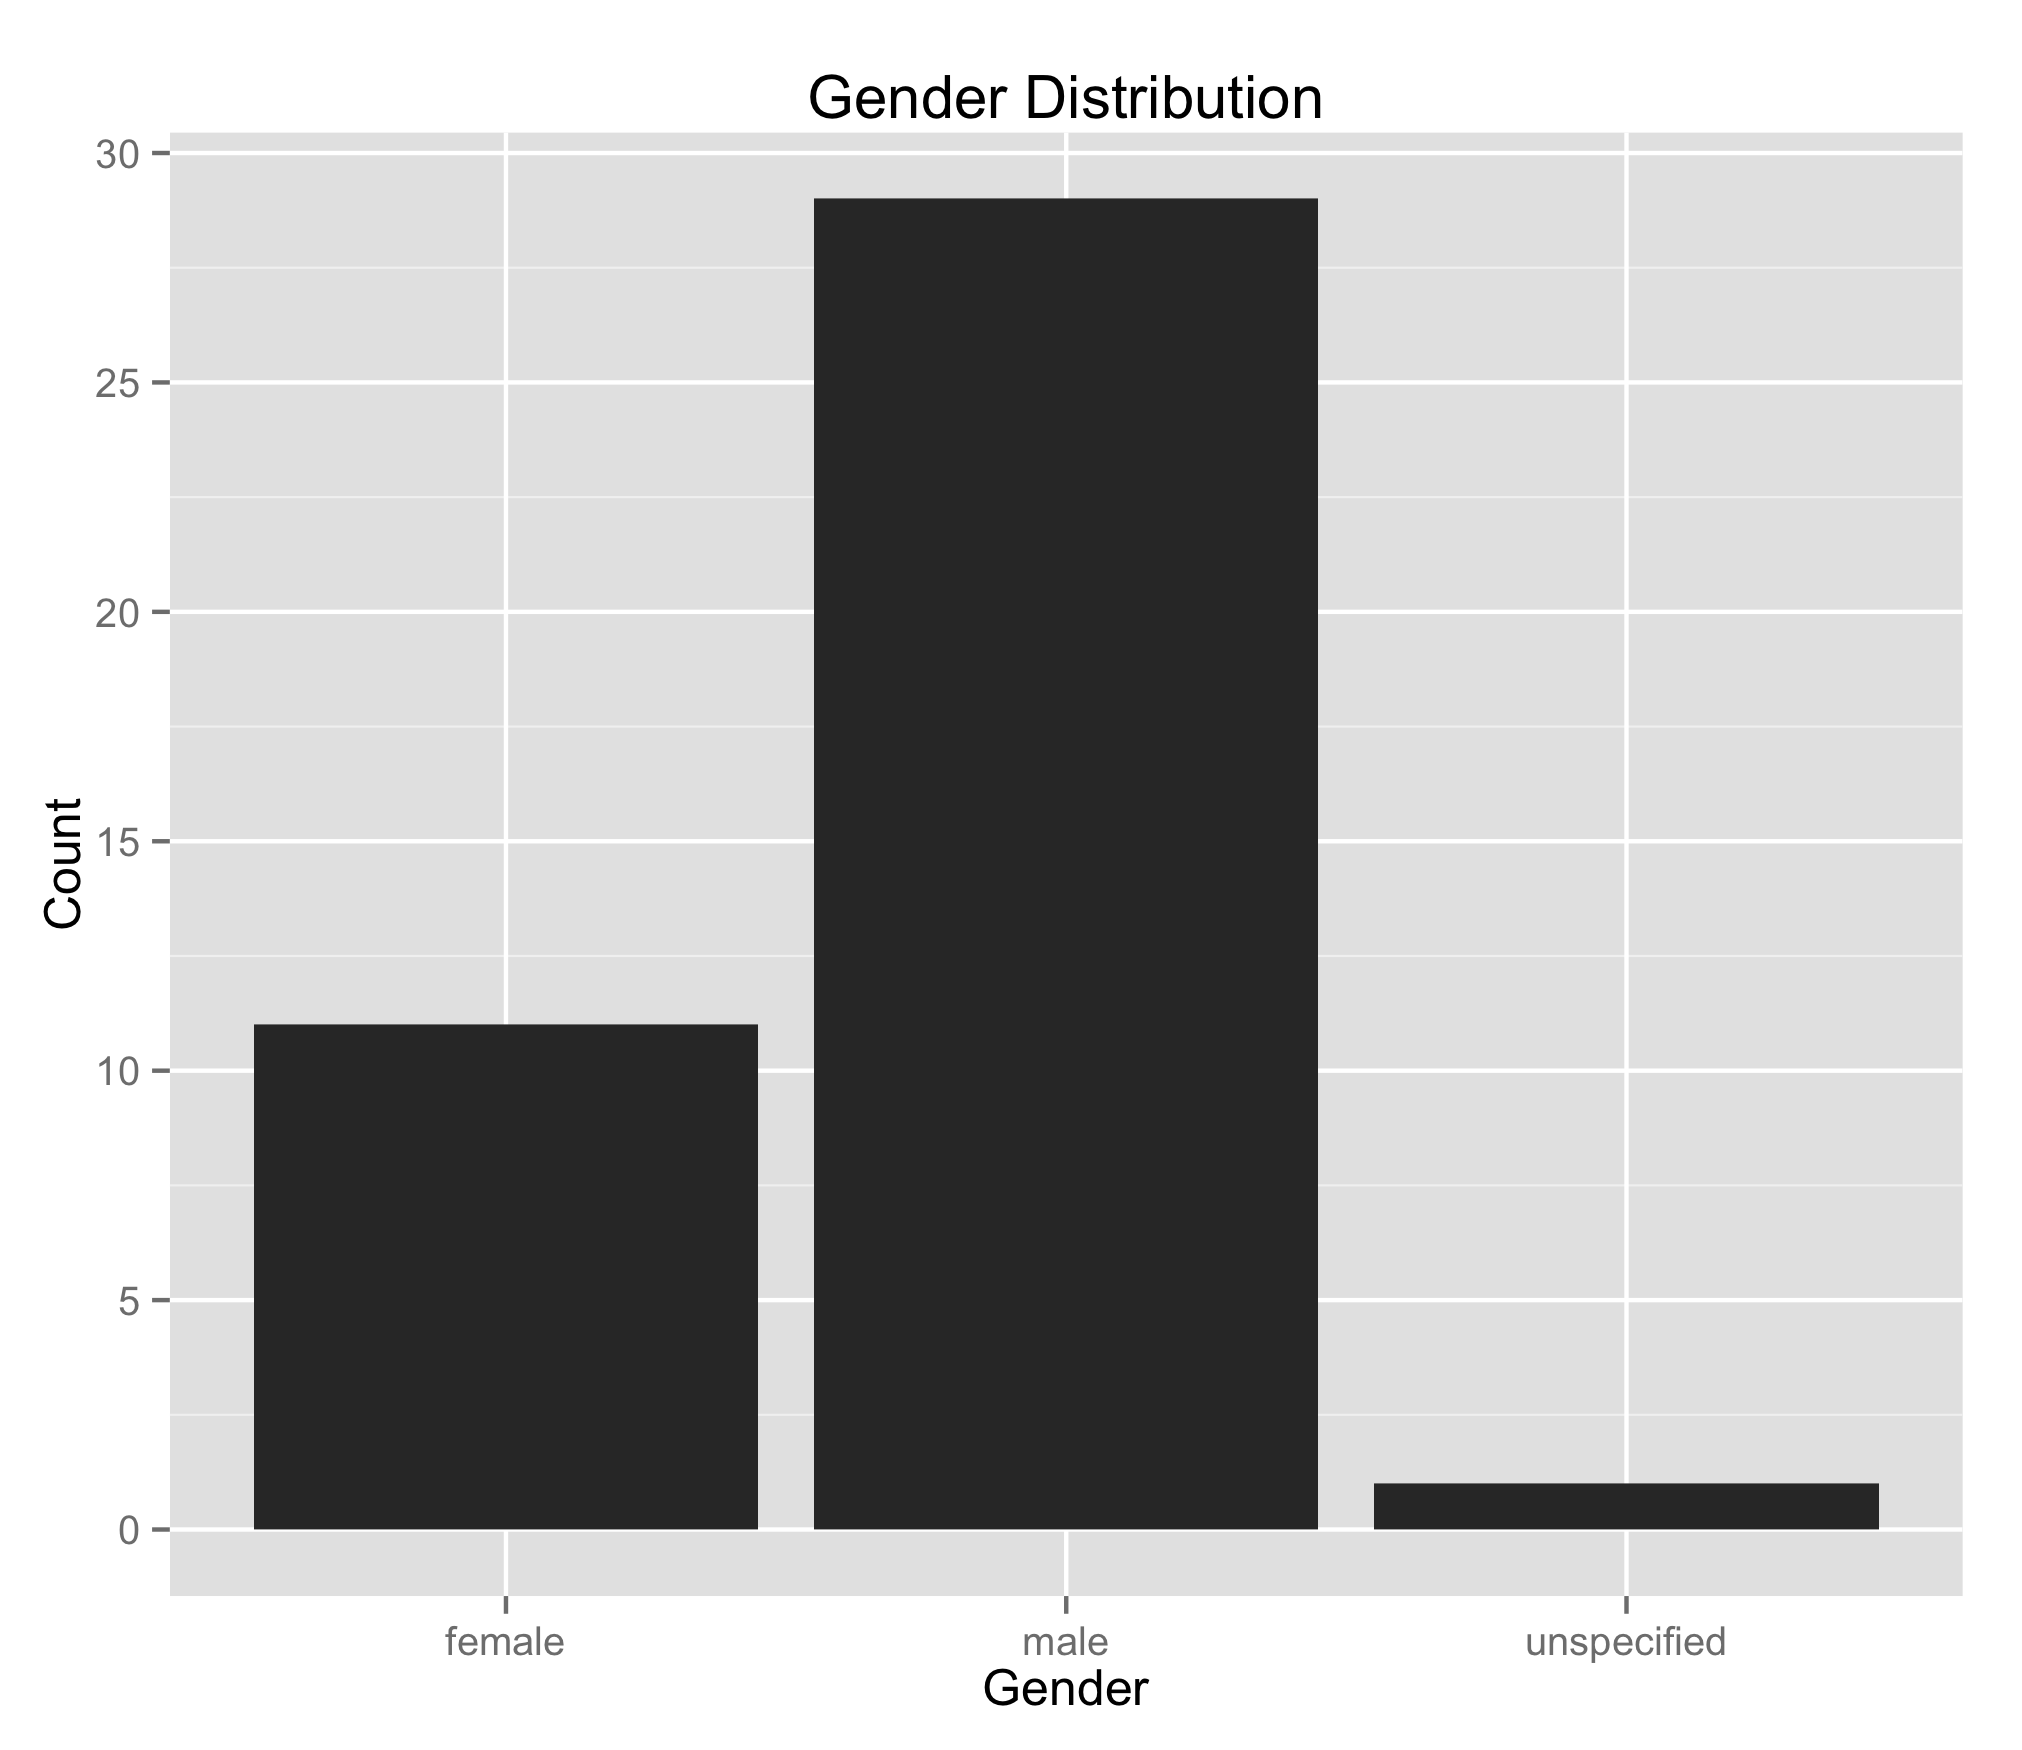
\includegraphics[width=1.0\linewidth]{graphs/gender.png}
    \caption{Gender Distribution}
    \label{genderdistribution}
\end{subfigure}
\caption{Basic Demographics}
\end{figure}


\begin{figure}[t]
\centering
\begin{subfigure}{.5\textwidth}
    \centering
    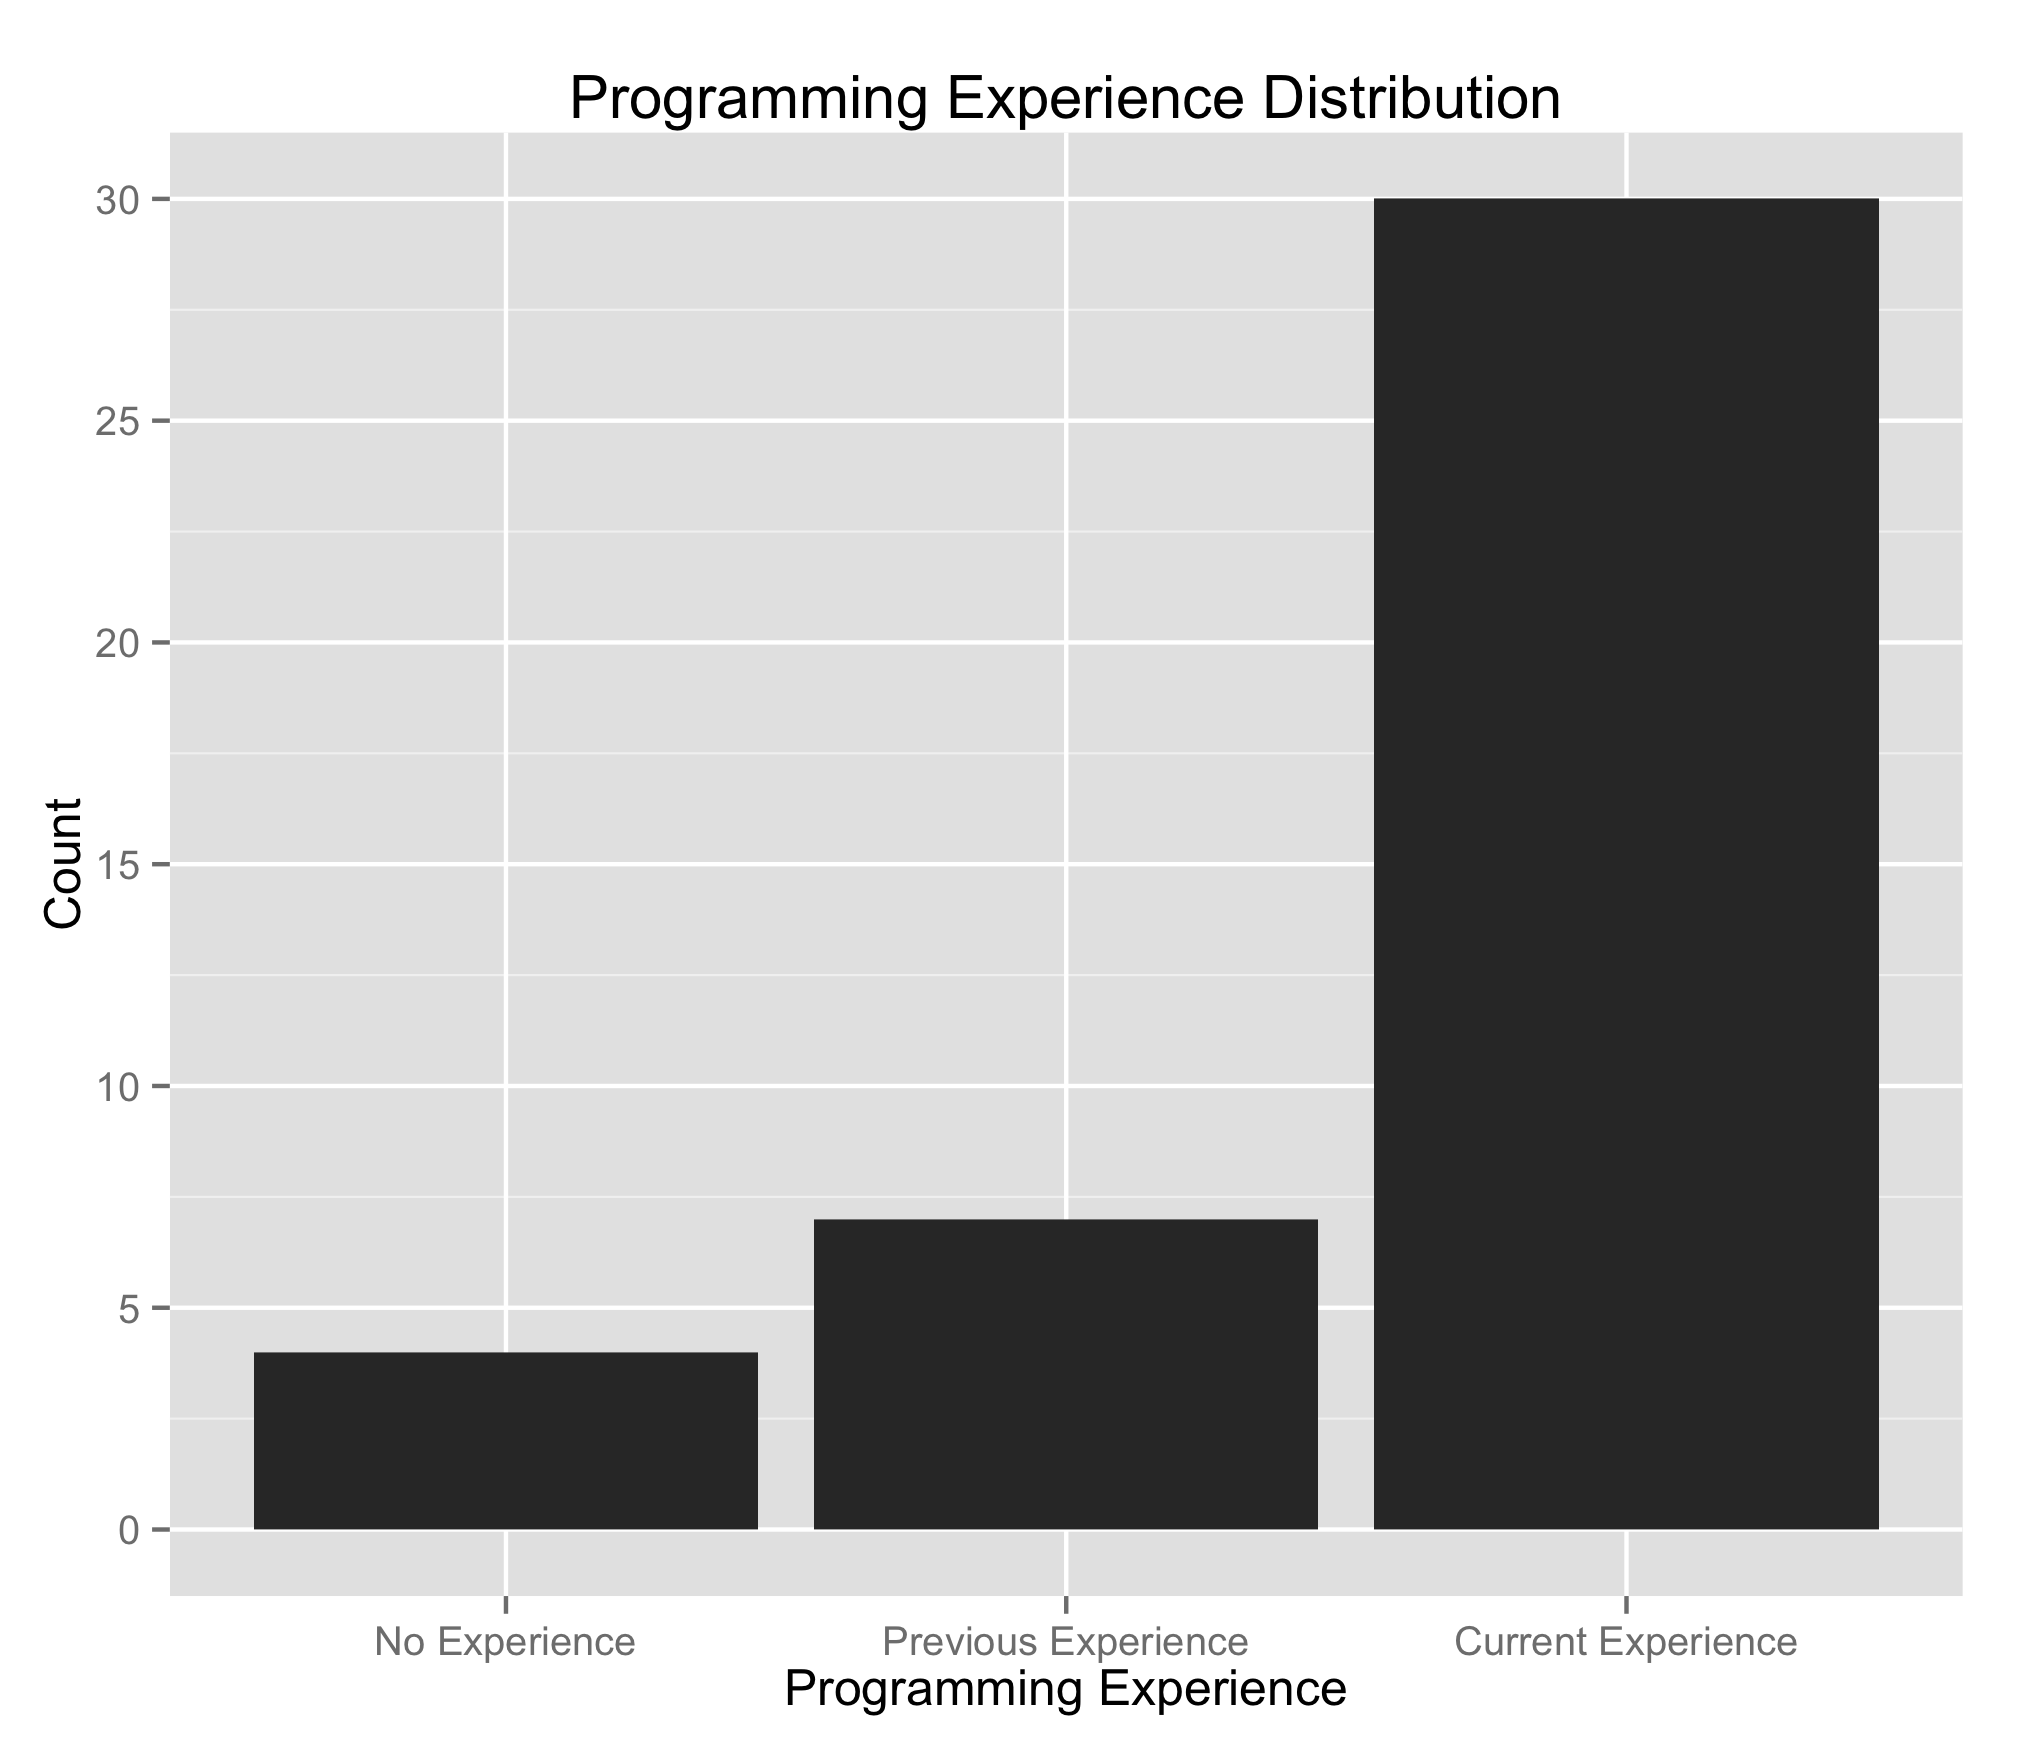
\includegraphics[width=1.0\linewidth]{graphs/programming.png}
    \caption{Programming Experience Distribution}
    \label{programmingdistribution}
\end{subfigure}%
\begin{subfigure}{.5\textwidth}
    \centering
    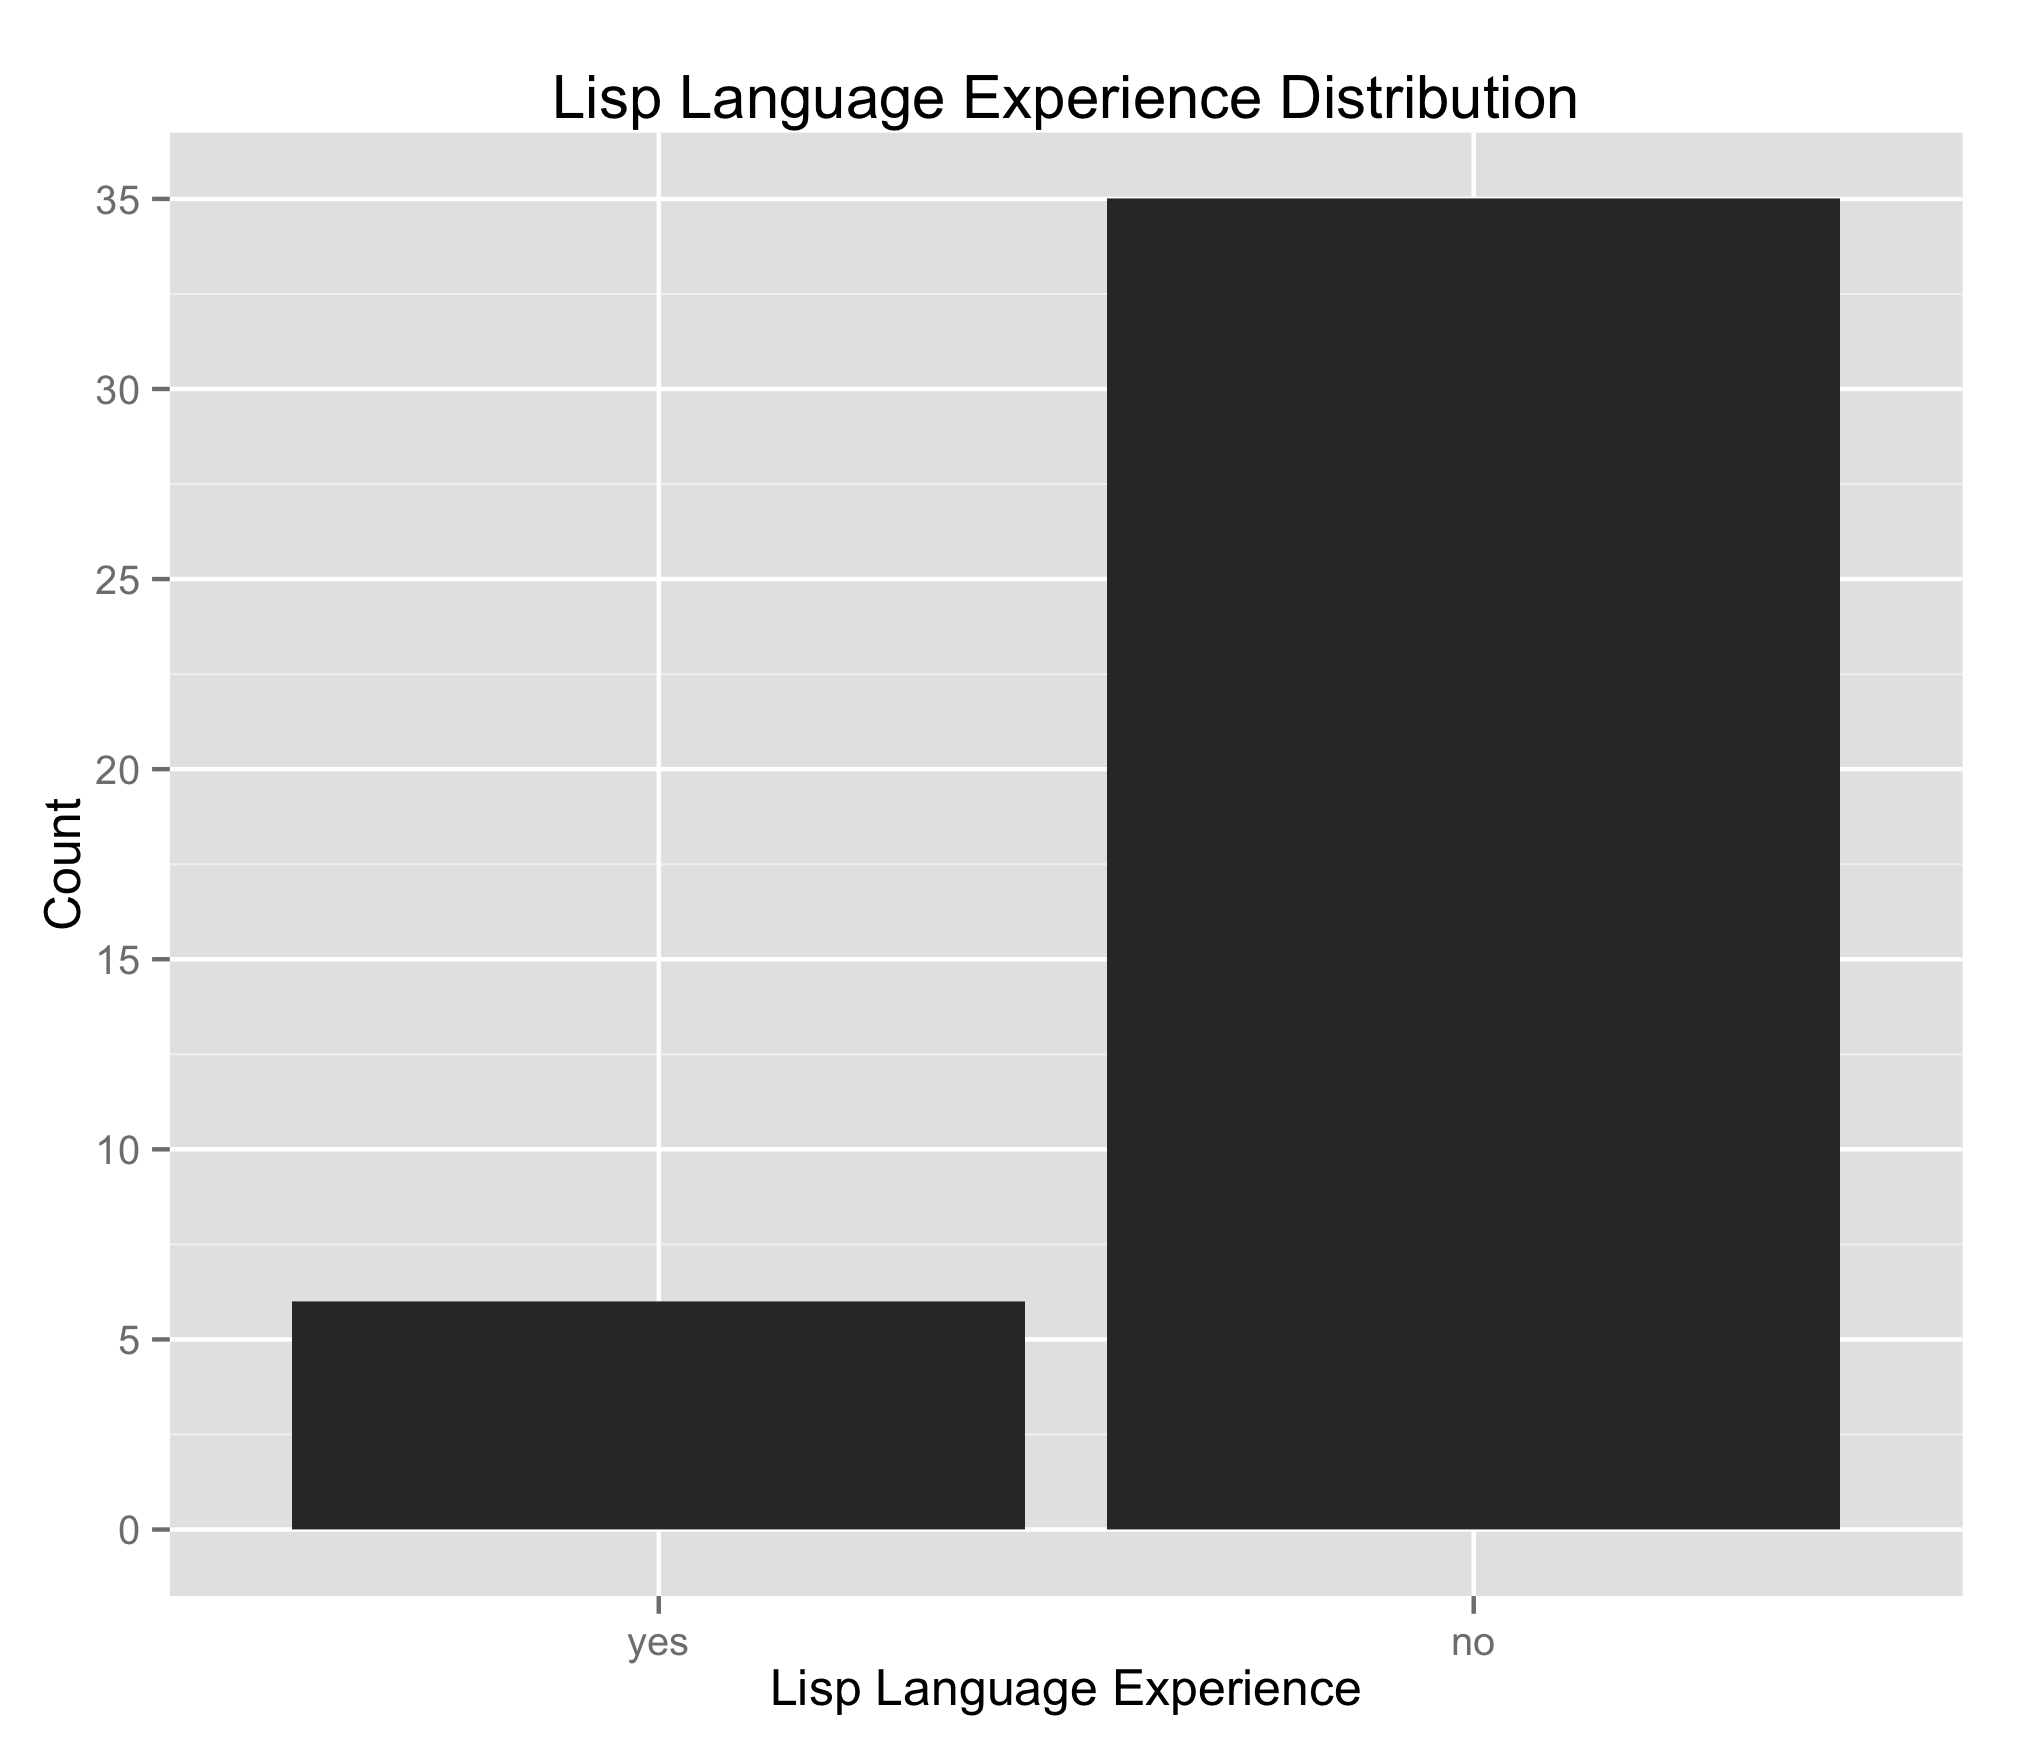
\includegraphics[width=1.0\linewidth]{graphs/lisp.png}
    \caption{Lisp Experience Distribution}
    \label{lispdistribution}
\end{subfigure}
\caption{Programming Demographics}
\end{figure}


\begin{figure}[t]
\centering
\begin{subfigure}{.5\textwidth}
    \centering
    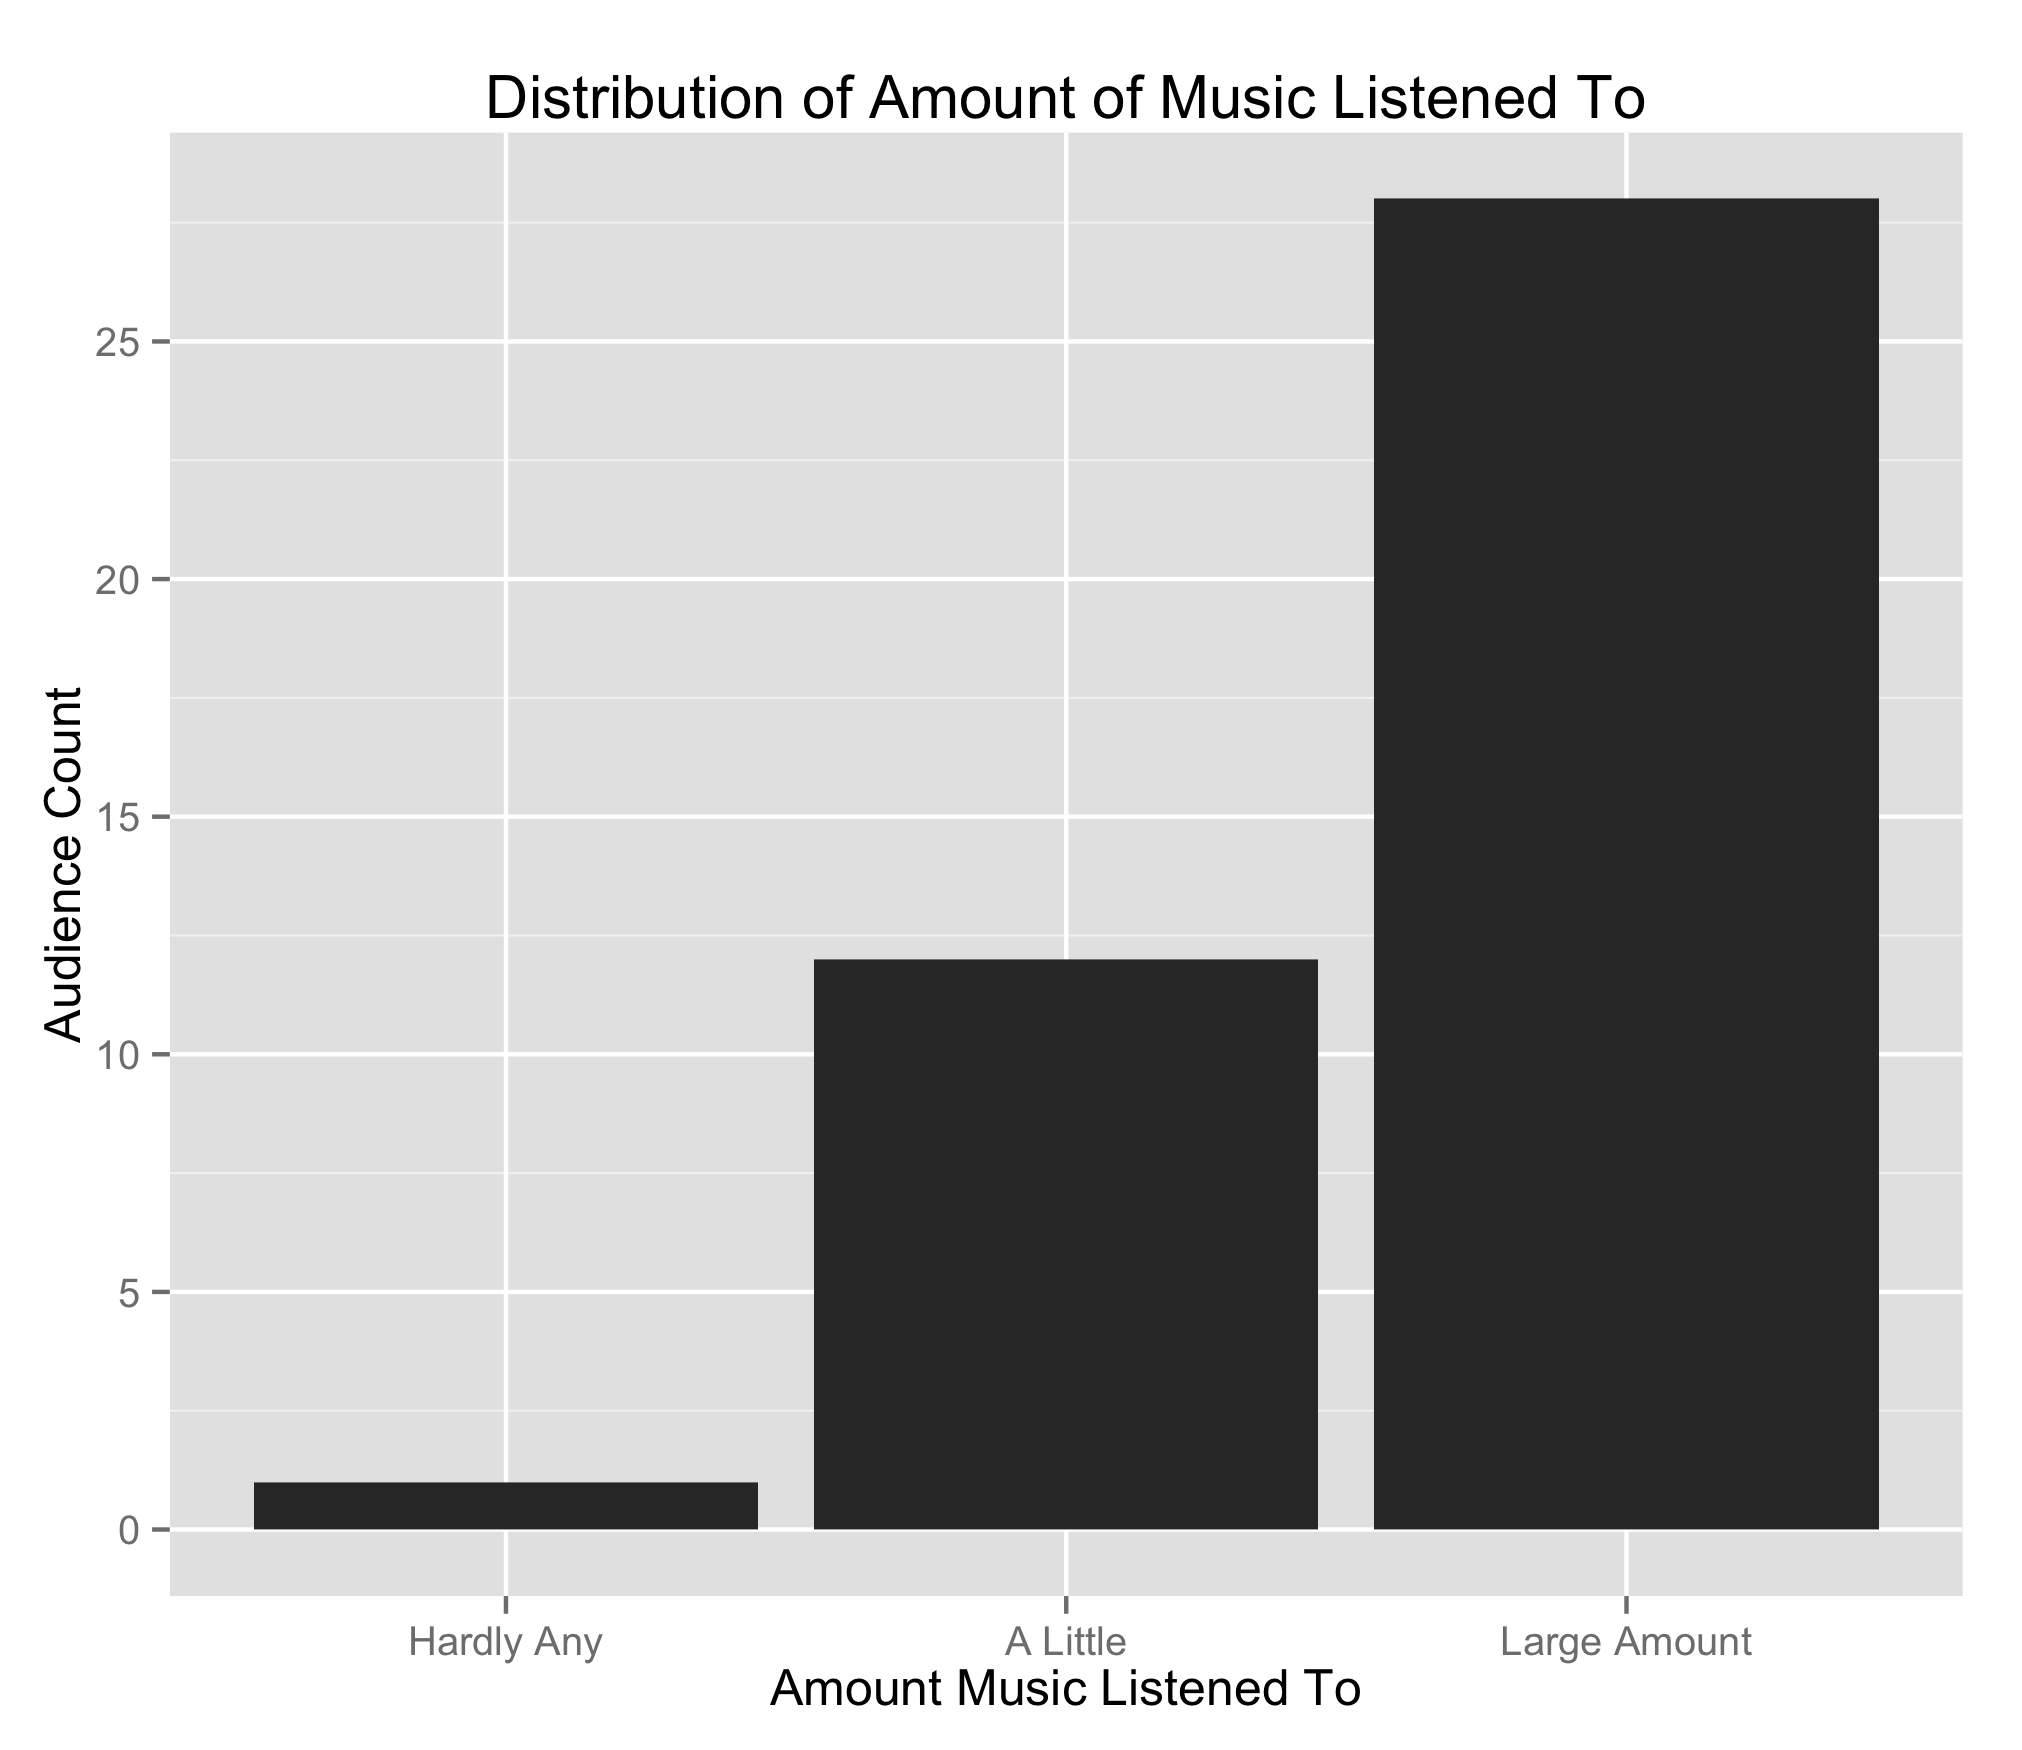
\includegraphics[width=1.0\linewidth]{graphs/music.png}
    \caption{Listen to Music Regularity Distribution}
    \label{musicdistribution}
\end{subfigure}%
\begin{subfigure}{.5\textwidth}
    \centering
    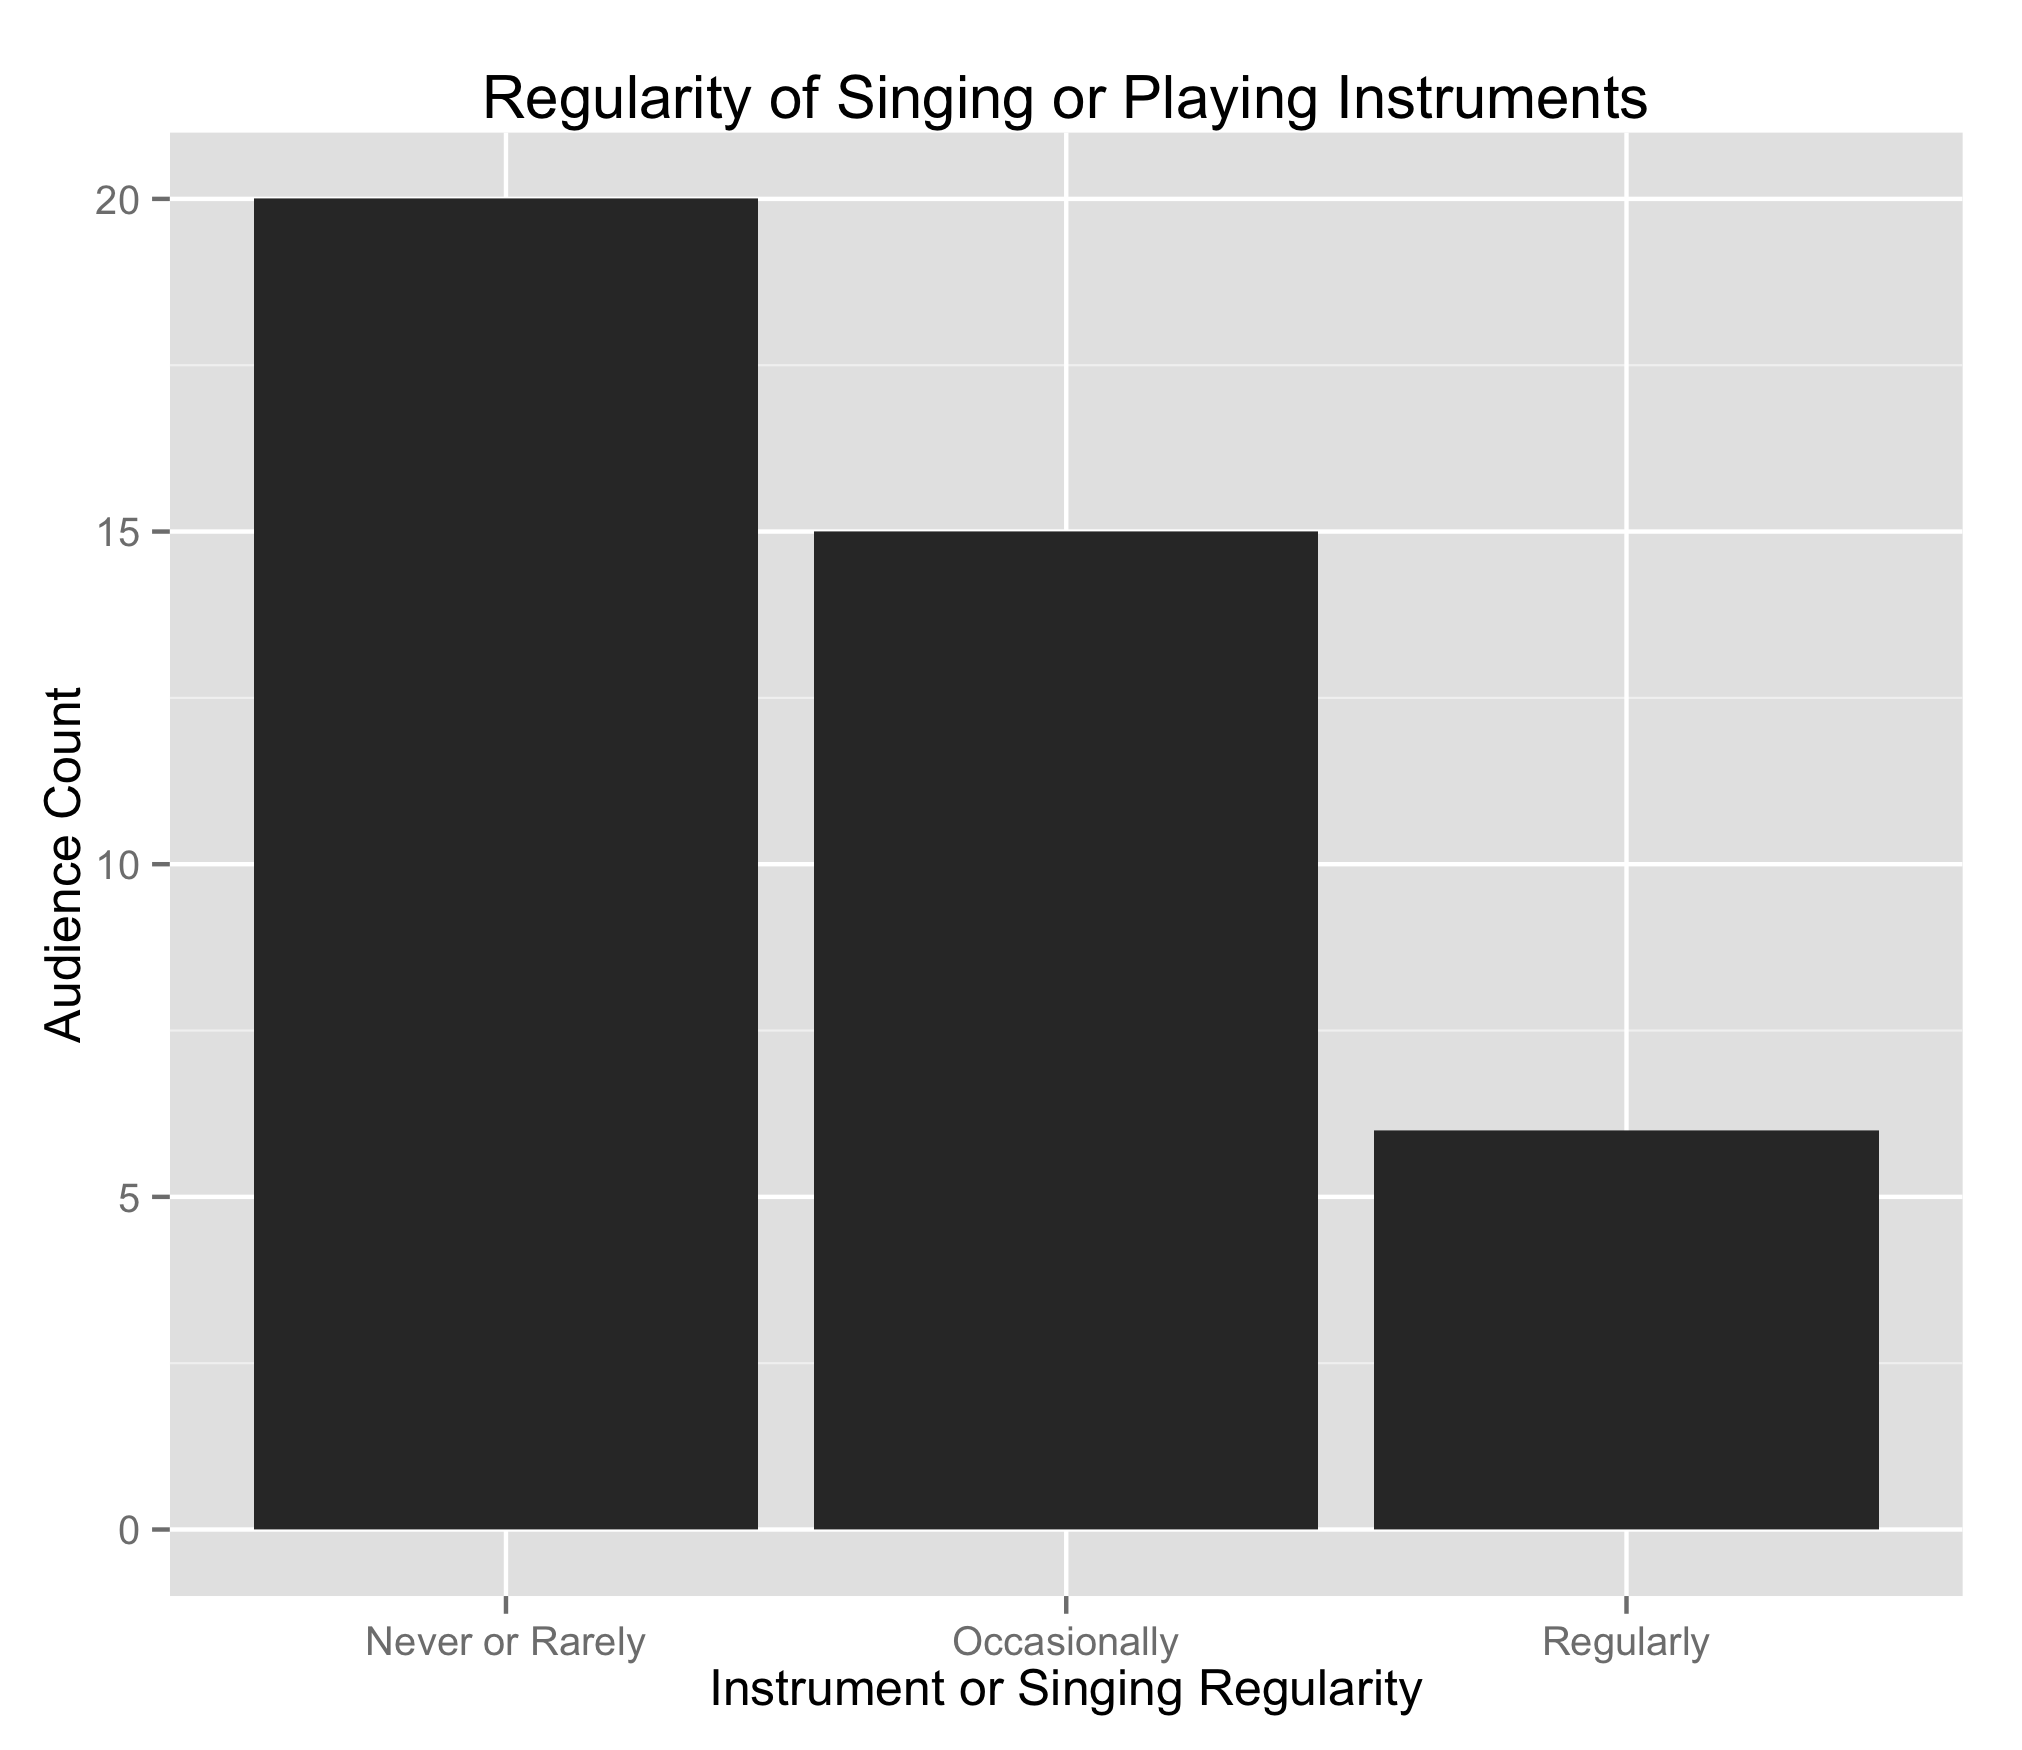
\includegraphics[width=1.0\linewidth]{graphs/instrument-regularity.png}
    \caption{Playing Instrument or Singing Regularity Distribution}
    \label{instrumentdistribution}
\end{subfigure}
\caption{Musical Demographics}
\end{figure}

\section{Results}

\subsection{Aesthetic vs Didactic Visualisation}

Understanding and enjoyment were evaluated against the didactic and aesthetic visualisations. Understanding and enjoyment trends throughout the performance are available in Table \ref{tab:understandtrend} and Table \ref{tab:enjoytrend}. Results and statistical analysis of the differences between the aesthetic and didactic conditions follows. Note that for the following statistical analysis a significance level of $0.05$ was used with the chi-squared test for independence.\\

\subsubsection{Understanding}
Overall, $37\%$ participants stated specifically that the didactic visualisations helped them to understand the code, whereas $12\%$ participants stated that the aesthetic visualisations assisted in understanding the code. See Table \ref{tab:helpunderstand} for the distribution of understanding between the aesthetic and didactic visualisations.\\

$H_0$: There is no difference between the aesthetic visualisations and didactic visualisations in terms of understanding.\\
$H_1$: There is a difference between the two visualisations in terms of understanding.\\

Significant difference between the visualisations effect on understanding were found ($\chi^2=7.1986,df=2,p=0.02734$).

\subsubsection{Enjoyment}
Overall, for both visualisations, a large proportion ($> 50\%$) of the participants stated that the visualisations helped their enjoyment of the performance. Of the participants, $76\%$ stated that the aesthetic visualisations helped their enjoyment compared to $56\%$ participants that stated the didactic visualisations helped their enjoyment. See Table \ref{tab:helpenjoy} for the distribution of enjoyment between the aesthetic and didactic visualisations.\\

$H_0$: There is no difference between the aesthetic visualisations and didactic visualisations in terms of enjoyment.\\
$H_1$: There is a difference between the two visualisations in terms of enjoyment.\\

No significant difference between the two visualisations effect on enjoyment were found ($\chi^2=3.7733,df=2,p=0.1516$).

\subsubsection{Liveness}


\subsection{Improvements}


\section{Discussion}

The response to the aesthetic visualisation [...more discussion to come]\\

[data indicates that aesthetic reduced early drop in enjoyment]\\

[didactic response]\\

In general, the visualisations contribution to enjoyment was fairly positive. This was the case for both visualisations. For understanding however, only the didactic visualisation assisted understanding during the performance.\\

[understanding discussion]\\

[understanding had the same pattern of understanding throughout the performance despite the starting differences]\\

[enjoyment discussion]\\

[difference between the two studies?]\\

[contribution of demographics to examined factors]\\

[qualitative data for improvement discussion]\\


A number of participants stated that the didactic visualisations were distracting, too abrupt or took away from the code in other ways. On the other hand, some said that the didactic visualisations gave the performance a sense of being 'too polished'. The general consensus, however, was that the visualisation should either better reflect the code, better reflect the music or have more variety.\\

[qualitative data for liveness discussion]\\

[what results will be used from this study]\\

[summarising thoughts]\\

\section{References}


@book{ware2013information,
  title={Information visualization: perception for design},
  author={Ware, Colin},
  year={2013},
  publisher={Elsevier}
}

@article{najjar1998principles,
  title={Principles of educational multimedia user interface design},
  author={Najjar, Lawrence J},
  journal={Human Factors: The Journal of the Human Factors and Ergonomics Society},
  volume={40},
  number={2},
  pages={311--323},
  year={1998},
  publisher={SAGE Publications}
}


\end{document}